\documentclass[a4paper,11pt]{article}

\usepackage[french]{babel}
\usepackage[T1]{fontenc}
\usepackage[utf8]{inputenc}
\usepackage{graphicx}
\usepackage{hyperref}
%\usepackage{fullpage}

\begin{document}

\author{Bazia Vincent\\Castanié Thibaut\\\textit{M2 IMAGINA}}
\title{\textbf{Cahier des charges jeu sérieux}\\Urban Wheelchair}
\date{5 novembre 2015}

\maketitle

\newpage

L’objectif de notre projet est de développer un jeu sérieux de sensibilisation à propos des difficultés que rencontrent les personnes en fauteuil roulant dans un milieu urbain non aménagé. 

Ce projet sera réalisé avec l’unité d’enseignement Sons et Musique.

\section{Outils}
Pour réaliser notre jeu, nous utiliserons le moteur \textbf{Unity 3D}. Afin de réaliser les sons et la musique, nous utiliserons \textbf{LMMS}, ainsi que \textbf{FMOD} et son plug-in Unity pour les intégrer dans le moteur. Enfin, pour travailler en collaboration, nous utiliserons le système de versions \textbf{Git}, ainsi que des outils de communication vocale à distance.

\section{Gameplay}

\subsection*{Synopsis}

Combinaison entre deux cœurs de jeu :
\begin{itemize}
\item Course : Atteindre un but le plus rapidement possible.
\item Construction : Modifier les éléments qui gênent le joueur avec un équipement adapté. 
\end{itemize}

Le joueur contrôle un personnage en fauteuil roulant dans le monde inadapté et doit essayer de l’améliorer en modifiant certains obstacles.

\subsection*{Contrôles}

Le joueur utilise les touches fléchées et la souris pour se déplacer dans l’environnement à la première personne. Le joueur peut avancer, reculer et pivoter son fauteuil à droite et à gauche.
Il utilise la souris en mode plan et clique sur les éléments à modifier.

Il y a deux vues différentes pour nos deux phases de jeu: 
\begin{itemize}
\item Vue 3D mobile à la première personne pour le contrôle de la personne en fauteuil roulant.
\item Vue 3D statique de dessus pour modifier les éléments.
\end{itemize}

\subsection*{Mécanismes}
\paragraph{Boucle O-C-R}
\begin{itemize}
\item \textit{Objectif} : Terminer le parcours dans un temps imparti
\item \textit{Challenge} : Le parcours n’est pas adapté pour une personne en fauteuil roulant.
\item \textit{Récompense} : Une fois un niveau réussi, on a accès au suivant.
\item \textit{Moyens} : Le joueur peut modifier certains éléments du parcours afin d’améliorer son temps. (remplacement d’escaliers, ascenseur, ...)
\end{itemize}

\subsection*{Règles du jeu}

Le joueur est propulsé aux commandes d’un fauteuil roulant. Il doit alors se déplacer dans un environnement urbanisé inadapté pour ses déplacements. Son but est d’aller d’un point A à un point B dans un temps donné. Sur son parcours il va devoir faire face à de nombreux obstacles. Certains d’entre eux vont le ralentir et l’agacer, tandis que d’autres seront infranchissables, devront être contournés et vont donc faire perdre beaucoup de temps. Une fois la première tentative effectuée, le joueur peut accéder au mode plan du parcours et acheter des équipements pour franchir les obstacles. Il doit cependant surveiller le budget qui lui est alloué et prendre les mesures nécessaires.

\subsection*{Assistance}

Au premier lancement des différentes phases de jeu, on présente les objectifs et les moyens d’y parvenir.
Les éléments qui peuvent être modifiés sont en surbrillances pendant la phase de construction.

\subsection*{\textit{Feedback}}
Le fauteuil roulant produit des sons différents en fonction de son mouvement. Le personnage exprime son mécontentement face aux obstacles. Lorsqu’un moyen adapté est installé, il exprime son contentement. Un son dans le style "récompense" est joué lorsque le parcours est fait dans les temps, un son d’échec sinon.

\subsection*{Menu}

Le jeu comporte un menu d’accueil basique pour lancer le jeu et effectuer d’éventuels réglages. En mode déplacement, un chrono montre le temps passé dans le niveau. En mode plan les éléments modifiables sont mis en avant et un clic sur l’un d’eux ouvre un menu permettant de choisir l’équipement à installer. Un menu permettant de recommencer ou de quitter la partie est disponible (en appuyant sur [Echap]).

\subsection*{Level Design}

Les niveaux du jeu se situent dans un milieu urbain composé d’obstacles modifiables.
Obstacles possibles :
\begin{itemize}
\item Escalier sans rampe d’accès
\item Sol (instable, glissant, impraticable, mauvais état, saletés)
\item Des axes de passages encombrés (travaux, obstacles ...)
\item Trottoir (trop étroit, trop haut)
\item Pentes trop brutes
\end{itemize}

Informations à propos des normes :\\\href{http://fauteuil-roulant.comprendrechoisir.com/comprendre/accessibilite-fauteuil-roulant}{fauteuil-roulant.comprendrechoisir.com/comprendre/accessibilite-fauteuil-roulant}

\section{Histoire}
Julie a passé la majeure partie de sa vie immobilisée sur un fauteuil roulant. Récemment, elle décide de s’impliquer dans la vie de sa commune dont les équipements ne sont pas du tout adaptés aux personnes dans son cas. Ravi de pouvoir améliorer le quotidien de ses habitants, le maire décide de lui accorder subvention afin qu’elle puisse se charger de choisir quels emplacements ou accès sont à améliorer afin de permettre leur fréquentation par des personnes en fauteuil.

\section{Analyse de l'existant}

Il n’existe actuellement pas de jeu sérieux visant à sensibiliser au handicap moteur. En revanche, la sensibilisation à d’autres types de handicaps (visuels, auditifs, vocaux) existe.

\subsection{Les secrets d'Ombyliss}

Ce jeu aurait pu être le premier jeu du marché à introduire les difficultés des personnes utilisant un fauteuil roulant à se déplacer dans un environnement inadapté. Seulement le jeu n’est jamais sorti car sa campagne de financement participatif n’a pas abouti. Son analyse sera donc basée sur la présentation faite sur sa page Ulule.

\begin{center}
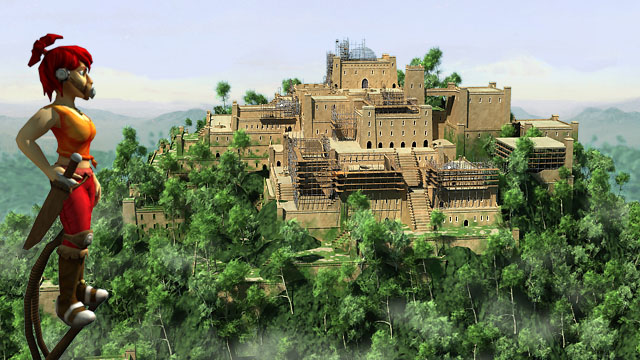
\includegraphics[scale=0.45]{./fig/jeu1.png}
\end{center}

Il s’agit d’un jeu de type \textit{point-and-click}, dans un environnement 3D où le joueur doit contrôler l’héroïne, Fairhom, pour l’aider à améliorer l’accessibilité dans la cité d’Ombyliss. Le jeu reprend plusieurs types de handicaps, mais le handicap moteur est mis en avant, de par la taille de l’héroïne qui est bien trop petite par rapport aux installations de la ville.

Le but de ce jeu sérieux est de sensibiliser les jeunes de 10 à 14 ans à une perception différente de la personne handicapée, afin qu’ils puissent en parler en classe ou dans des groupes de discussion, et aborder le sujet du handicap avec un œil neuf. En effet, le terme "handicap" porte encore aujourd’hui une connotation négative, c’est pour cela que les développeurs du jeu ont décidé d’en parler, sans y faire référence. Ainsi, l’aventure se déroule dans un univers fantastique, où il existes plusieurs espèces qui possèdent des caractéristiques et des capacités diversifiées.

\subsection{A Blind Legend}

A Blind Legend est un jeu pour mobiles entièrement basé sur le son. A l'aide d'un procédé reproduisant la perception du son dans un environnement en 3D, le joueur progresse en se fiant seulement à ses oreilles, via quelques gestes sur l’écran de son smartphone. 

\begin{center}
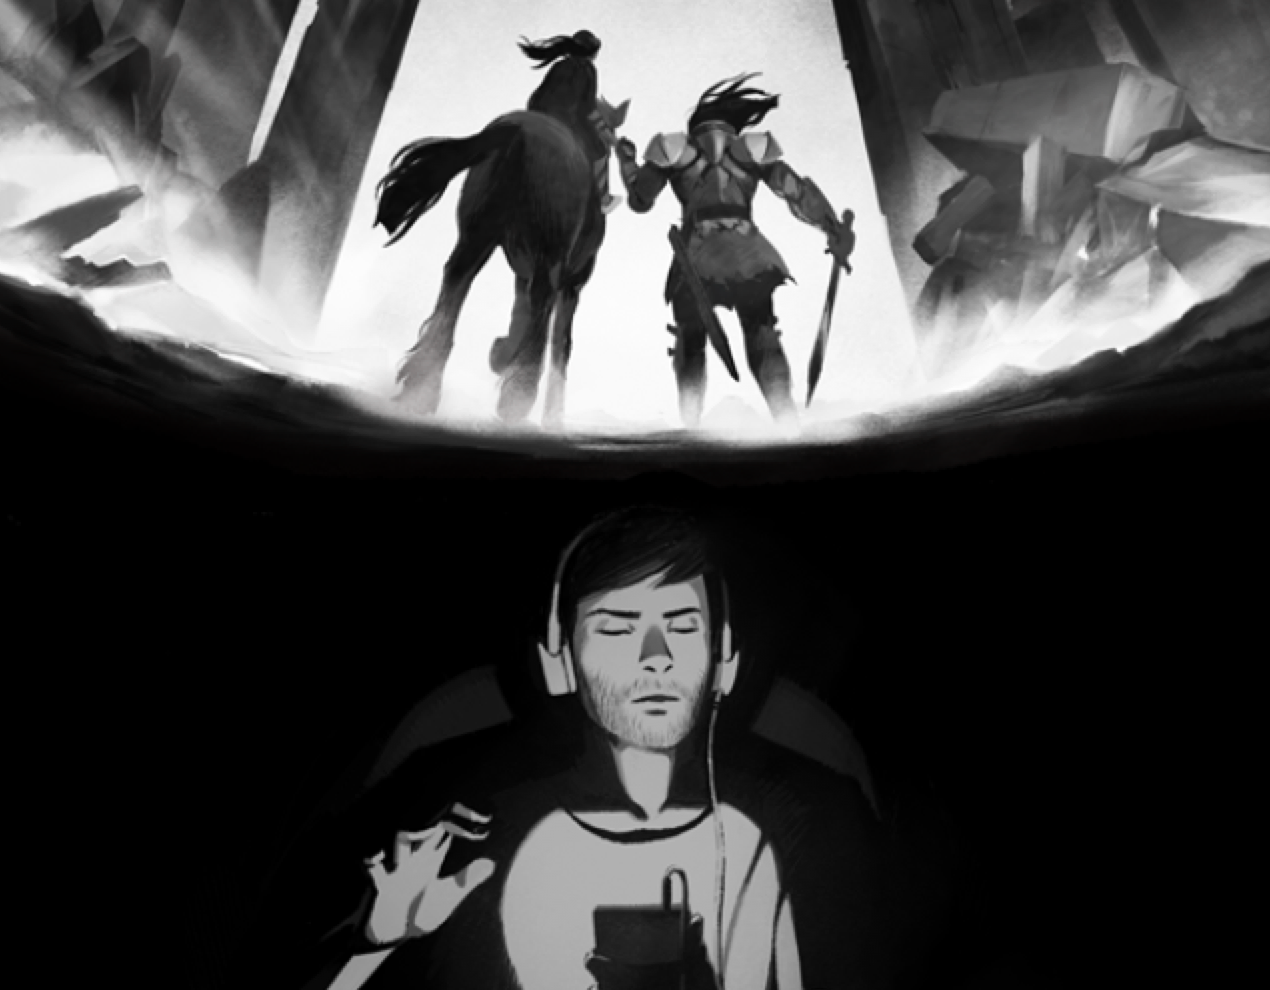
\includegraphics[scale=0.4]{./fig/jeu2.png}
\end{center}

Le joueur est dans la peau d’un chevalier aveugle, à l’époque du Moyen-âge. Il est aidé dans sa quête par la voix de sa fille, qui guide le joueur sur la direction à suivre tout au long de l’aventure. Il faut ainsi un temps d’adaptation pour ne plus se fier simplement à sa vue, mais faire confiance à son ouïe. Le jeu consiste en des phases d’explorations, des phases de "QTE auditifs" et des phases de combat. Pendant les phases d’explorations, le joueur est plongé dans un environnement sonore riche et doit suivre la voix de la fille. Pour cela, un \textit{tap} simple permet de l’entendre nous appeler. On peut alors se déplacer dans la directions souhaitée en faisant glisser son doigt sur l’écran à partir de son centre. Une fois la destination de sa fille atteinte, elle se déplace jusqu’à une nouvelle destination. En se déplaçant, le joueur entend le bruit de ses propres pas, de ceux de sa fille, mais aussi de multiples autres sources sonores comme le vent dans les feuillages, le bruit d’un chariot, le caquètement de poules... Pendant les phases de QTE, le joueur fait face à des évènements tels une chute de pierres ou une poursuite à cheval qui testent les réflexes. Enfin les phases de combats consistent à tendre l’oreille pour déterminer la position de l’adversaire afin de bloquer ses coups et de contre-attaquer.

La technologie du jeu permet d’accentuer l’effet stéréo, et l’utilisation d’un casque ou d’écouteurs est donc nécessaire. Il est aussi conseillé de fermer les yeux et de s’isoler pour une meilleure expérience. Après avoir passé un certain temps dans le jeu, on est surpris de ne plus faire confiance qu’aux sons et bruits qui nous entourent. Même si cela n’est pas explicitement dit dans le jeu, cela permet de nous sensibiliser aux personnes possédant un handicap visuel. On constate facilement qu’il est très difficile de se déplacer et de se repérer sans une aide extérieure. De plus l’imagination joue un rôle très important, on se met rapidement à imaginer le paysage qui nous entoure, seulement au bruit du vent dans les feuillages, au bruit de ses pas sur les chemins de terre ou pavés; les apparences des personnages de l’aventure sont aussi propres à notre imagination, en fonction du timbre de leur voix, de la résonance de leur pas...

Ce jeu identifie donc le handicap en mettant directement le joueur dans la peau d’un personnage aveugle. Cela permet d’avoir un aperçu de ce que peut être la vie d’un handicapé visuel, tout en gardant le côté ludique et scénaristique d’un jeu d’aventure.

\subsection{Le silence d'Aquari}

Le silence d'Aquari est un jeu de type \textit{point-and-click} où le joueur est propulsé aux commandes d’un personnage qui s’éveille au sein d’une cité peuplée d’habitants malentendants, qui utilisent la langue des signes pour communiquer entre eux.

\begin{center}
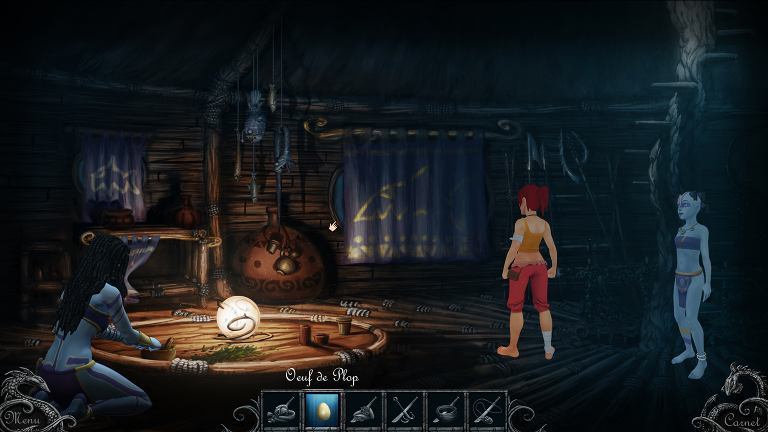
\includegraphics[scale=0.35]{./fig/jeu3.png}
\end{center}

Le jeu est ouvert à des enfants à partir de 8 ans, afin de les sensibiliser au handicap auditif. En effet, la particularité du gameplay réside dans le fait que ce soit l’héroïne qui est en situation de handicap par rapport aux autres personnages. C’est la seule qui est "entendante" dans une cité composée d’habitants malentendants. Ainsi, en inversant la position entre la personne handicapée et non-handicapée, on pousse le joueur à changer sa perception par rapport à cette thématique, vu qu’il ne connaît pas la langue des signes.

Une fois de plus, ce jeu sensibilise le joueur par une mise en situation. En effet, il comprend la difficulté ressentie lorsqu’il faut s’adapter à un moyen de communication qui n’est pas le sien.


\end{document}